\documentclass[./00PhotoBox.tex]{subfiles}
\graphicspath{{\subfix{./img/}}}
\begin{document}


\chapter{Aufbau des Messsystems}
\label{c:aufbau}
Entsprechend der im \autoref{c:photogrammetrie} beschriebenen Anforderungen an ein photogrammetrisches Messsystem wurden die Komponenten ausgewählt.

Die Kameras sollten eine hohe geometrische Auflösung und möglichst stabile \gls{innereOrientierung} aufweisen. Außerdem sollen sie während einer Messkampagne nicht in ihrer Lage zueinander verändert werden, damit die \gls{aeussereOrientierung} größtenteils gleich bleibt. Daher ist ein stabiler Rahmen notwendig, an welchem die Kameras verdrehsicher angebracht werden können. Kleinere Restfehler in den Orientierungen können mit der Bündelblockausgleichung ausgeglichen werden.
Um Ungenauigkeiten durch Bewegungen zu verhindern, müssen die Kameras möglichst zeitgleich auslösen. Daher ist eine gemeinsame Steuerung und Kommunikation zwischen den Kameras notwendig. Außerdem sollen alle Bilder auf das Steuerungssystem übertragen werden, hierfür wird eine Form der Datenübertragung benötigt. Damit die Bilder möglichst schattenfrei ausgeleuchtet werden, muss eine Beleuchtung mit eingeplant werden. Außerdem muss die Stromversorgung der einzelnen Kameras sichergestellt sein.

In diesem Kapitel wird der Aufbau des Messsystems beschrieben und die Auswahl der Komponenten begründet.

\section{Kameras}
\label{s:kameras}
Als Kameras wurde das Raspberry Pi Camera Module 3 verwendet, welches jeweils von einem Raspberry Pi Zero W gesteuert wird. Im Vergleich zu anderen günstigen Kameras wie Webcams oder der ESP32 CAM haben die Kameras eine hohe geometrische Auflösung von 12 Megapixeln und dennoch mit \SI{1,4}{\micro\metre} relativ große \acrfull{px} \citep{raspicamdatasheet}, was im subjektiven Eindruck eine sehr gute Bildqualität ergibt.

Andere Kameramodule für den Raspberry Pi wurden in \autoref{tab:vergleich_kameras} verglichen. Das Camera Module v1 entfiel als Möglichkeit, da die Kamera einen Mindestabstand von einem Meter benötigt. Hiermit müsste der Aufnahmebereich für die Objekte auf über zwei Meter vergrößert werden. Die HQ- und GS-Kameras haben kein Objektiv mitgeliefert, sodass hier die Kosten für ein Objektiv hinzukommen würden. Das Camera Module v2 hat eine geringere Auflösung und auch eine geringere Bildqualität bei gleichem Preis wie das Modul 3. Außerdem ist die Fokussierung nur manuell möglich, was die Automatisierung desselben verhindert. Das Camera Module 3 Wide hat zwar ein größeres Sichtfeld, jedoch damit auch eine geringere Auflösung auf dem Objekt. Vorteil ist der geringe Mindestabstand. Da das Camera Module 3 besser verfügbar und etwas günstiger war, wurde sich für dieses Modell entschieden, was einen guten Kompromiss aus Auflösung, Bildqualität und Preis darstellt.

\begin{table}
    \centering
    \caption{Vergleich der möglichen Kameramodule für den Raspberry Pi \citep{raspicamdatasheet}}
    \label{tab:vergleich_kameras}
    \resizebox{\textwidth}{!}{%
        \begin{tabular}{l|l|l|r|lr|r|l|r|}
            \cline{2-9}
                                                                & \textbf{Preis}               & \textbf{\begin{tabular}[c]{@{}l@{}}Sensor-\\ auflösung\end{tabular}} & \textbf{\begin{tabular}[c]{@{}l@{}}Pixel\\ {[}µm{]}\end{tabular}} & \multicolumn{2}{l|}{\textbf{Fokus}}                                         & \textbf{\begin{tabular}[c]{@{}l@{}}Brennweite\\ {[}mm{]}\end{tabular}}   & \textbf{Sichtfeld}       & \textbf{Blende}                                         \\ \hline
            \multicolumn{1}{|l|}{\textbf{Camera Module v1}}     & \$25                         & 2592 × 1944                                                          & 1,40                                                              & \multicolumn{1}{l|}{\cellcolor[HTML]{FFCCC9}fix}                            & \cellcolor[HTML]{FFCCC9}{\color[HTML]{000000} \SI{1}{\metre} - $\infty$} & 3,60                     & 54° x 41°                & F2.9                         \\ \hline
            \multicolumn{1}{|l|}{\textbf{Camera Module v2}}     & \$25                         & 3280 × 2464                                                          & 1,12                                                              & \multicolumn{1}{l|}{\cellcolor[HTML]{FFCCC9}manuell}                        & \SI{10}{\centi\metre} - $\infty$                                         & 3,04                     & 62° x 49°                & F2.0                         \\ \hline
            \multicolumn{1}{|l|}{\textbf{Camera Module 3}}      & \cellcolor[HTML]{9AFF99}\$25 & \cellcolor[HTML]{9AFF99}4608 x 2592                                  & 1,40                                                              & \multicolumn{1}{l|}{\cellcolor[HTML]{9AFF99}motorisiert}                    & \SI{10}{\centi\metre} - $\infty$                                         & 4,74                     & 66° x 41°                & \cellcolor[HTML]{9AFF99}F1.8 \\ \hline
            \multicolumn{1}{|l|}{\textbf{Camera Module 3 Wide}} & \$35                         & \cellcolor[HTML]{9AFF99}4608 x 2592                                  & 1,40                                                              & \multicolumn{1}{l|}{\cellcolor[HTML]{9AFF99}motorisiert}                    & \cellcolor[HTML]{9AFF99}\SI{5}{\centi\metre} - $\infty$                  & 2,75                     & 102° x 67°               & F2.2                         \\ \hline
            \multicolumn{1}{|l|}{\textbf{HQ Camera}}            & \cellcolor[HTML]{FFCCC9}\$50 & 4056 x 3040                                                          & 1,55                                                              & \multicolumn{1}{l|}{\cellcolor[HTML]{FFCCC9}{\color[HTML]{000000} manuell}} & \cellcolor[HTML]{C0C0C0}                                                 & \cellcolor[HTML]{C0C0C0} & \cellcolor[HTML]{C0C0C0} & \cellcolor[HTML]{C0C0C0}     \\ \hline
            \multicolumn{1}{|l|}{\textbf{GS Camera}}            & \cellcolor[HTML]{FFCCC9}\$50 & 1456 x 1088                                                          & \cellcolor[HTML]{9AFF99}3,45                                      & \multicolumn{1}{l|}{\cellcolor[HTML]{FFCCC9}{\color[HTML]{000000} manuell}} & \cellcolor[HTML]{C0C0C0}                                                 & \cellcolor[HTML]{C0C0C0} & \cellcolor[HTML]{C0C0C0} & \cellcolor[HTML]{C0C0C0}     \\ \hline
        \end{tabular}
    }
\end{table}

Nachteil und Vorteil zugleich ist, dass die Kamera über einen Autofokus verfügt, der aber auch elektronisch gesteuert manuell fokussieren kann. Dieser verschlechtert die Stabilität der inneren Orientierung und wurde daher im \autoref{c:voruntersuchungen} analysiert. Da die Bilder im Makrobereich zwischen \SI{0,1}{} und \SI{1}{\metre} aufgenommen werden und die Kameras keine Veränderung der Blende ermöglichen, ist die Schärfentiefe vergleichsweise niedrig. Hierauf wurde in den Untersuchungen in \autoref{sec:fokusstacking} genauer eingegangen.

Ein weiterer Vorteil der Lösung mit einzelnen Raspberry Pi besteht darin, dass hierdurch bereits die einzelnen Kameraeinheiten parallel zur Datenübertragung Aufgaben wie das Identifizieren von Passpunkten übernehmen können. Durch die Parallelisierung dieses Schrittes ist eine Reduktion der Berechnungszeit zwischen den Aufnahmen zu erwarten. Zudem ermöglicht die Nutzung von kabellosen Netzwerkverbindungen zur Steuerung eine Skalierung des Systems sowohl hinsichtlich der Anzahl der Kameras als auch der Abstände zwischen den Kameras.

Die Anzahl der Kameras für den Prototyp wurde zusammen mit der Art des Rahmens (siehe \autoref{s:rahmen}) definiert. Hierzu wurde der Rahmen mit seinen Kameras in der 3D-Visualisierungssoftware Blender modelliert und einzelne Bilder der möglichen Kamera-Positionen gerendert. Im Anschluss wurden die Bilder in Agisoft Metashape zur Berechnung eines 3D-Modells verwendet. Dabei wurde evaluiert, ob die Berechnung möglich ist und wie gut die Abdeckung des Testobjektes ist. Das virtuelle Modell des Systems wurde darüber hinaus genutzt, um Visualisierungen für die Bedienungsanleitung zu erstellen (siehe \autoref{ch:Bedienungsanleitung}). Eine Verwendung in der Websoftware zur visuellen Überprüfung der berechneten Kamera-Positionen wurde geprüft, aber nicht umgesetzt, da die Erkennbarkeit schlechter als erwartet war.

\section{Rahmen}
\label{s:rahmen}

\begin{figure}
    \centering
    \begin{subfigure}{0.30\textwidth}
        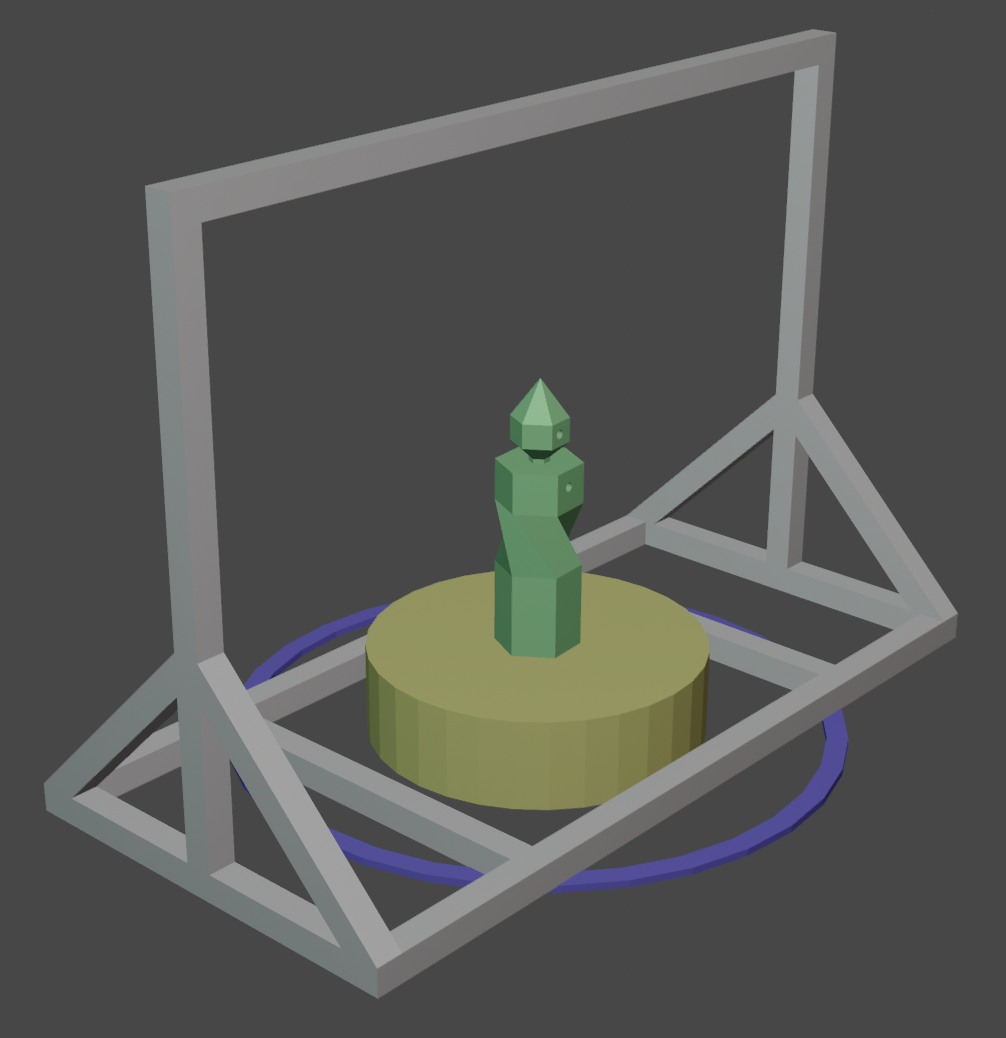
\includegraphics[height=1\linewidth]{./img/3_aufbau/modell1.png}
        \centering
        \caption{Unter Nutzung\\eines Drehtellers}
        \label{img:entwurf1}
    \end{subfigure}
    \begin{subfigure}{0.30\textwidth}
        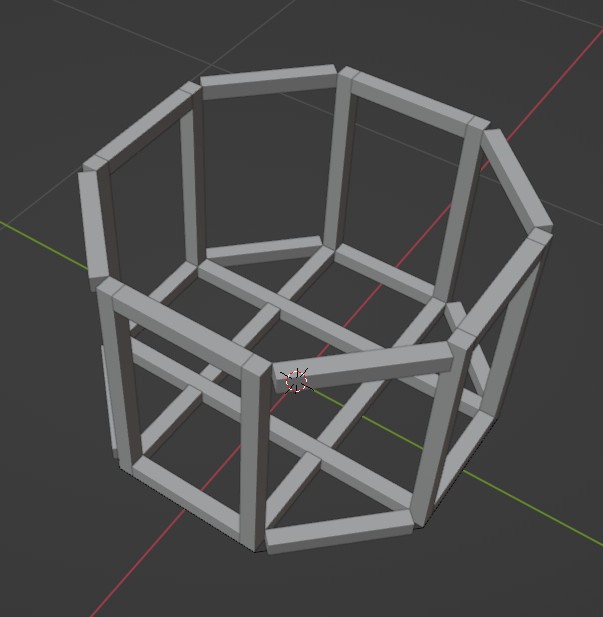
\includegraphics[height=1\linewidth]{./img/3_aufbau/modell2.png}
        \centering
        \caption{Rahmen mit\\Boden-Versteifung}
        \label{img:entwurf2}
    \end{subfigure}
    \begin{subfigure}{0.30\textwidth}
        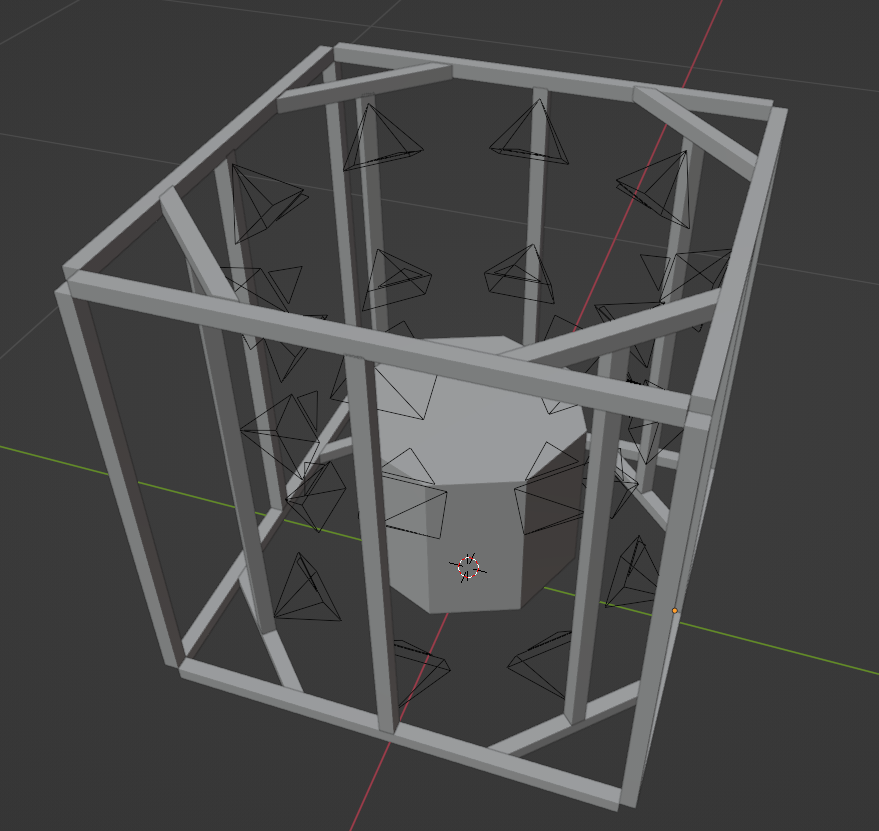
\includegraphics[height=1\linewidth]{./img/3_aufbau/modell3.png}
        \centering
        \caption{Endgültiger Entwurf mit seitlichen Versteifungen}
        \label{img:entwurf3}
    \end{subfigure}
    \caption{Verschiedene Entwurfsideen, modelliert mit Blender}
    \label{img:entwuerfe}
\end{figure}


Der Rahmen muss möglichst stabil sein, damit die Kameras sich nicht in ihrer Lage verändern können. Jedoch sollte das System auch weiterhin transportabel - also nicht zu schwer - und veränderbar bleiben, um beispielsweise Kameras für Messreihen in ihrer Lage zu verändern. Der Aufbau aus genormten Bauteilen bietet sich an, um hier ggf. den Nachbau einfach ermöglichen zu können. Außerdem sollte der Rahmen auch demontierbar sein, damit er transportiert werden kann.

Als mögliche Materialien kamen Holz, Stahl und Aluminium infrage. Aufgrund der einfachen Bearbeitung und der Standardisierung wurde sich für Aluminiumprofile entschieden. Diese gibt es in verschiedenen Ausführungen mit Nuten an den Seitenflächen, sodass eine einfache Montage, aber auch eine Demontage zu Transportzwecken, möglich wird. Außerdem sind diese sehr stabil bei leichtem Gewicht.


Es wurden verschiedene Varianten geprüft, die in \autoref{img:entwuerfe} dargestellt sind. Der erste Entwurf (siehe \autoref{img:entwurf1}) sah weniger Kameras und die zwingende Nutzung eines Drehtellers vor, dies wurde jedoch verworfen, weil dieser nicht der Anforderung einer schnellen Erfassung entsprochen hätte und auch der Anforderung der kurzen Einarbeitungszeit widersprechen würde. Der zweite Entwurf (siehe \autoref{img:entwurf2}) sah bereits die Nutzung von 8 Kamera-Hauptrichtungen vor, was für gute Schnittwinkel sorgt. Für die Aussteifung wurde hier ein Boden vorgesehen. Dies ist jedoch nachteilig, da das System dann beispielsweise nicht mehr über große, nicht bewegliche Objekte herüber gestülpt werden könnte. Gerade bei empfindlichen Objekten wäre dies aber vorteilhaft. In der dritten Variante (siehe \autoref{img:entwurf3}) wurde dann die Versteifung in den Seitenwänden umgesetzt. Durch die Konstruktion mit Eckwürfeln sowie der Bildung von dreieckigen Strukturen und dem Einbau von eckaussteifenden Platten mit Scheibenwirkung, wurde die Stabilität der Verbindungen erhöht. \autoref{img:alurahmen} zeigt den fertigen Rahmen vor Einbau der Platten und der Technik.


\begin{figure}
    \centering
    \begin{subfigure}{0.38\textwidth}
        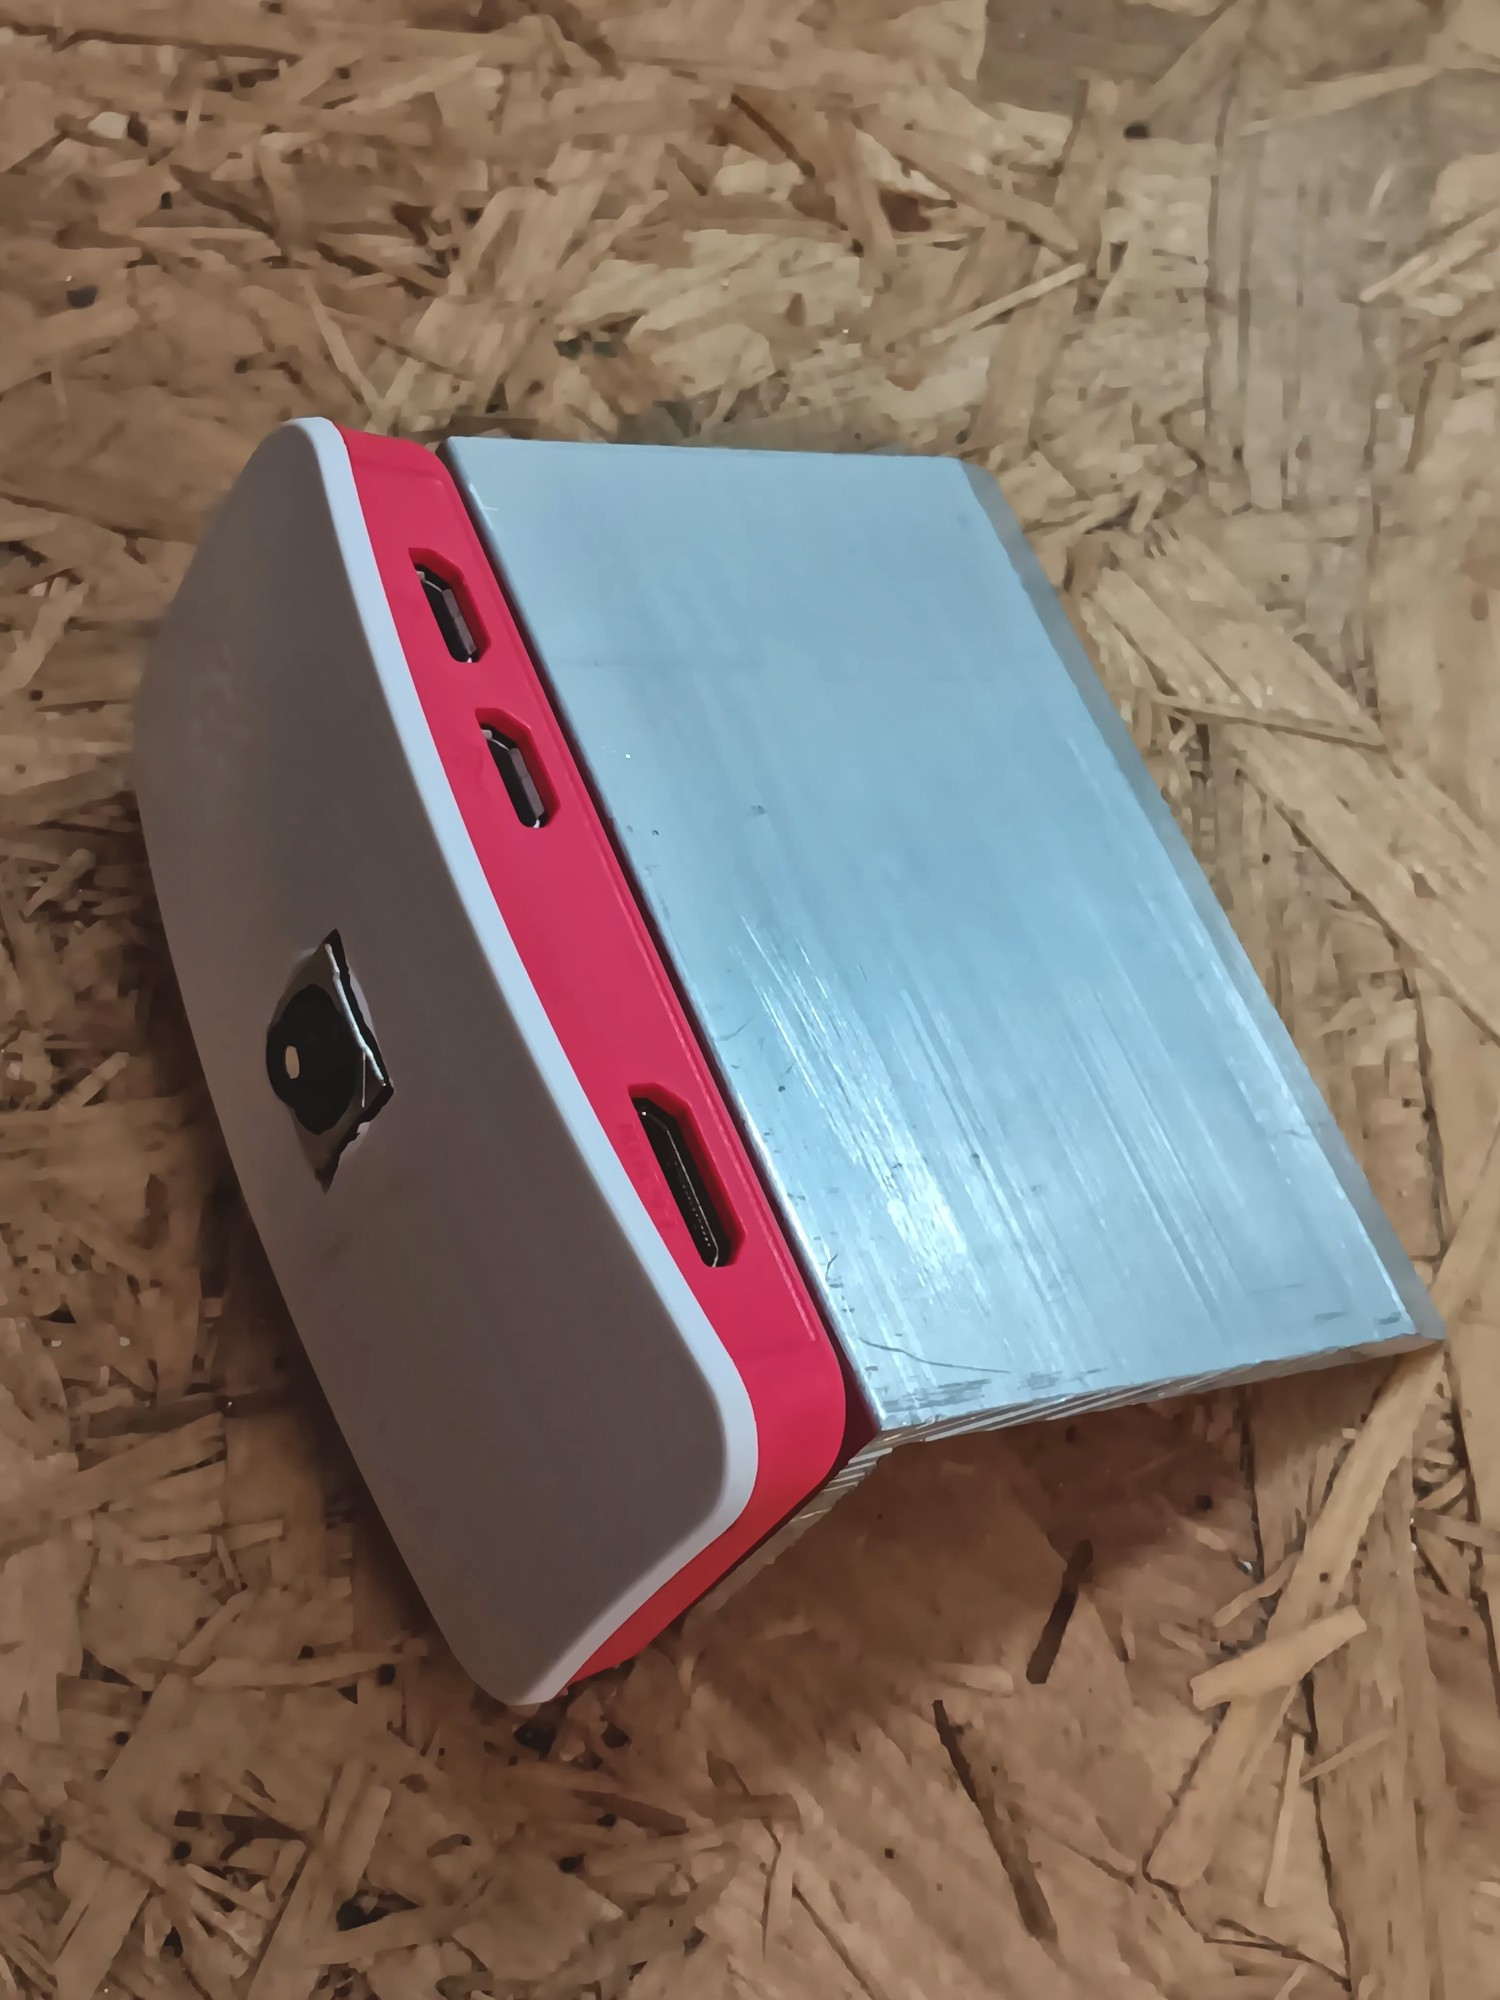
\includegraphics[height=6.5cm]{./img/3_aufbau/aluwinkel.jpg}
        \centering
        \caption{Kamera-Winkel}
        \label{img:aluwinkel}
    \end{subfigure}
    \begin{subfigure}{0.58\textwidth}
        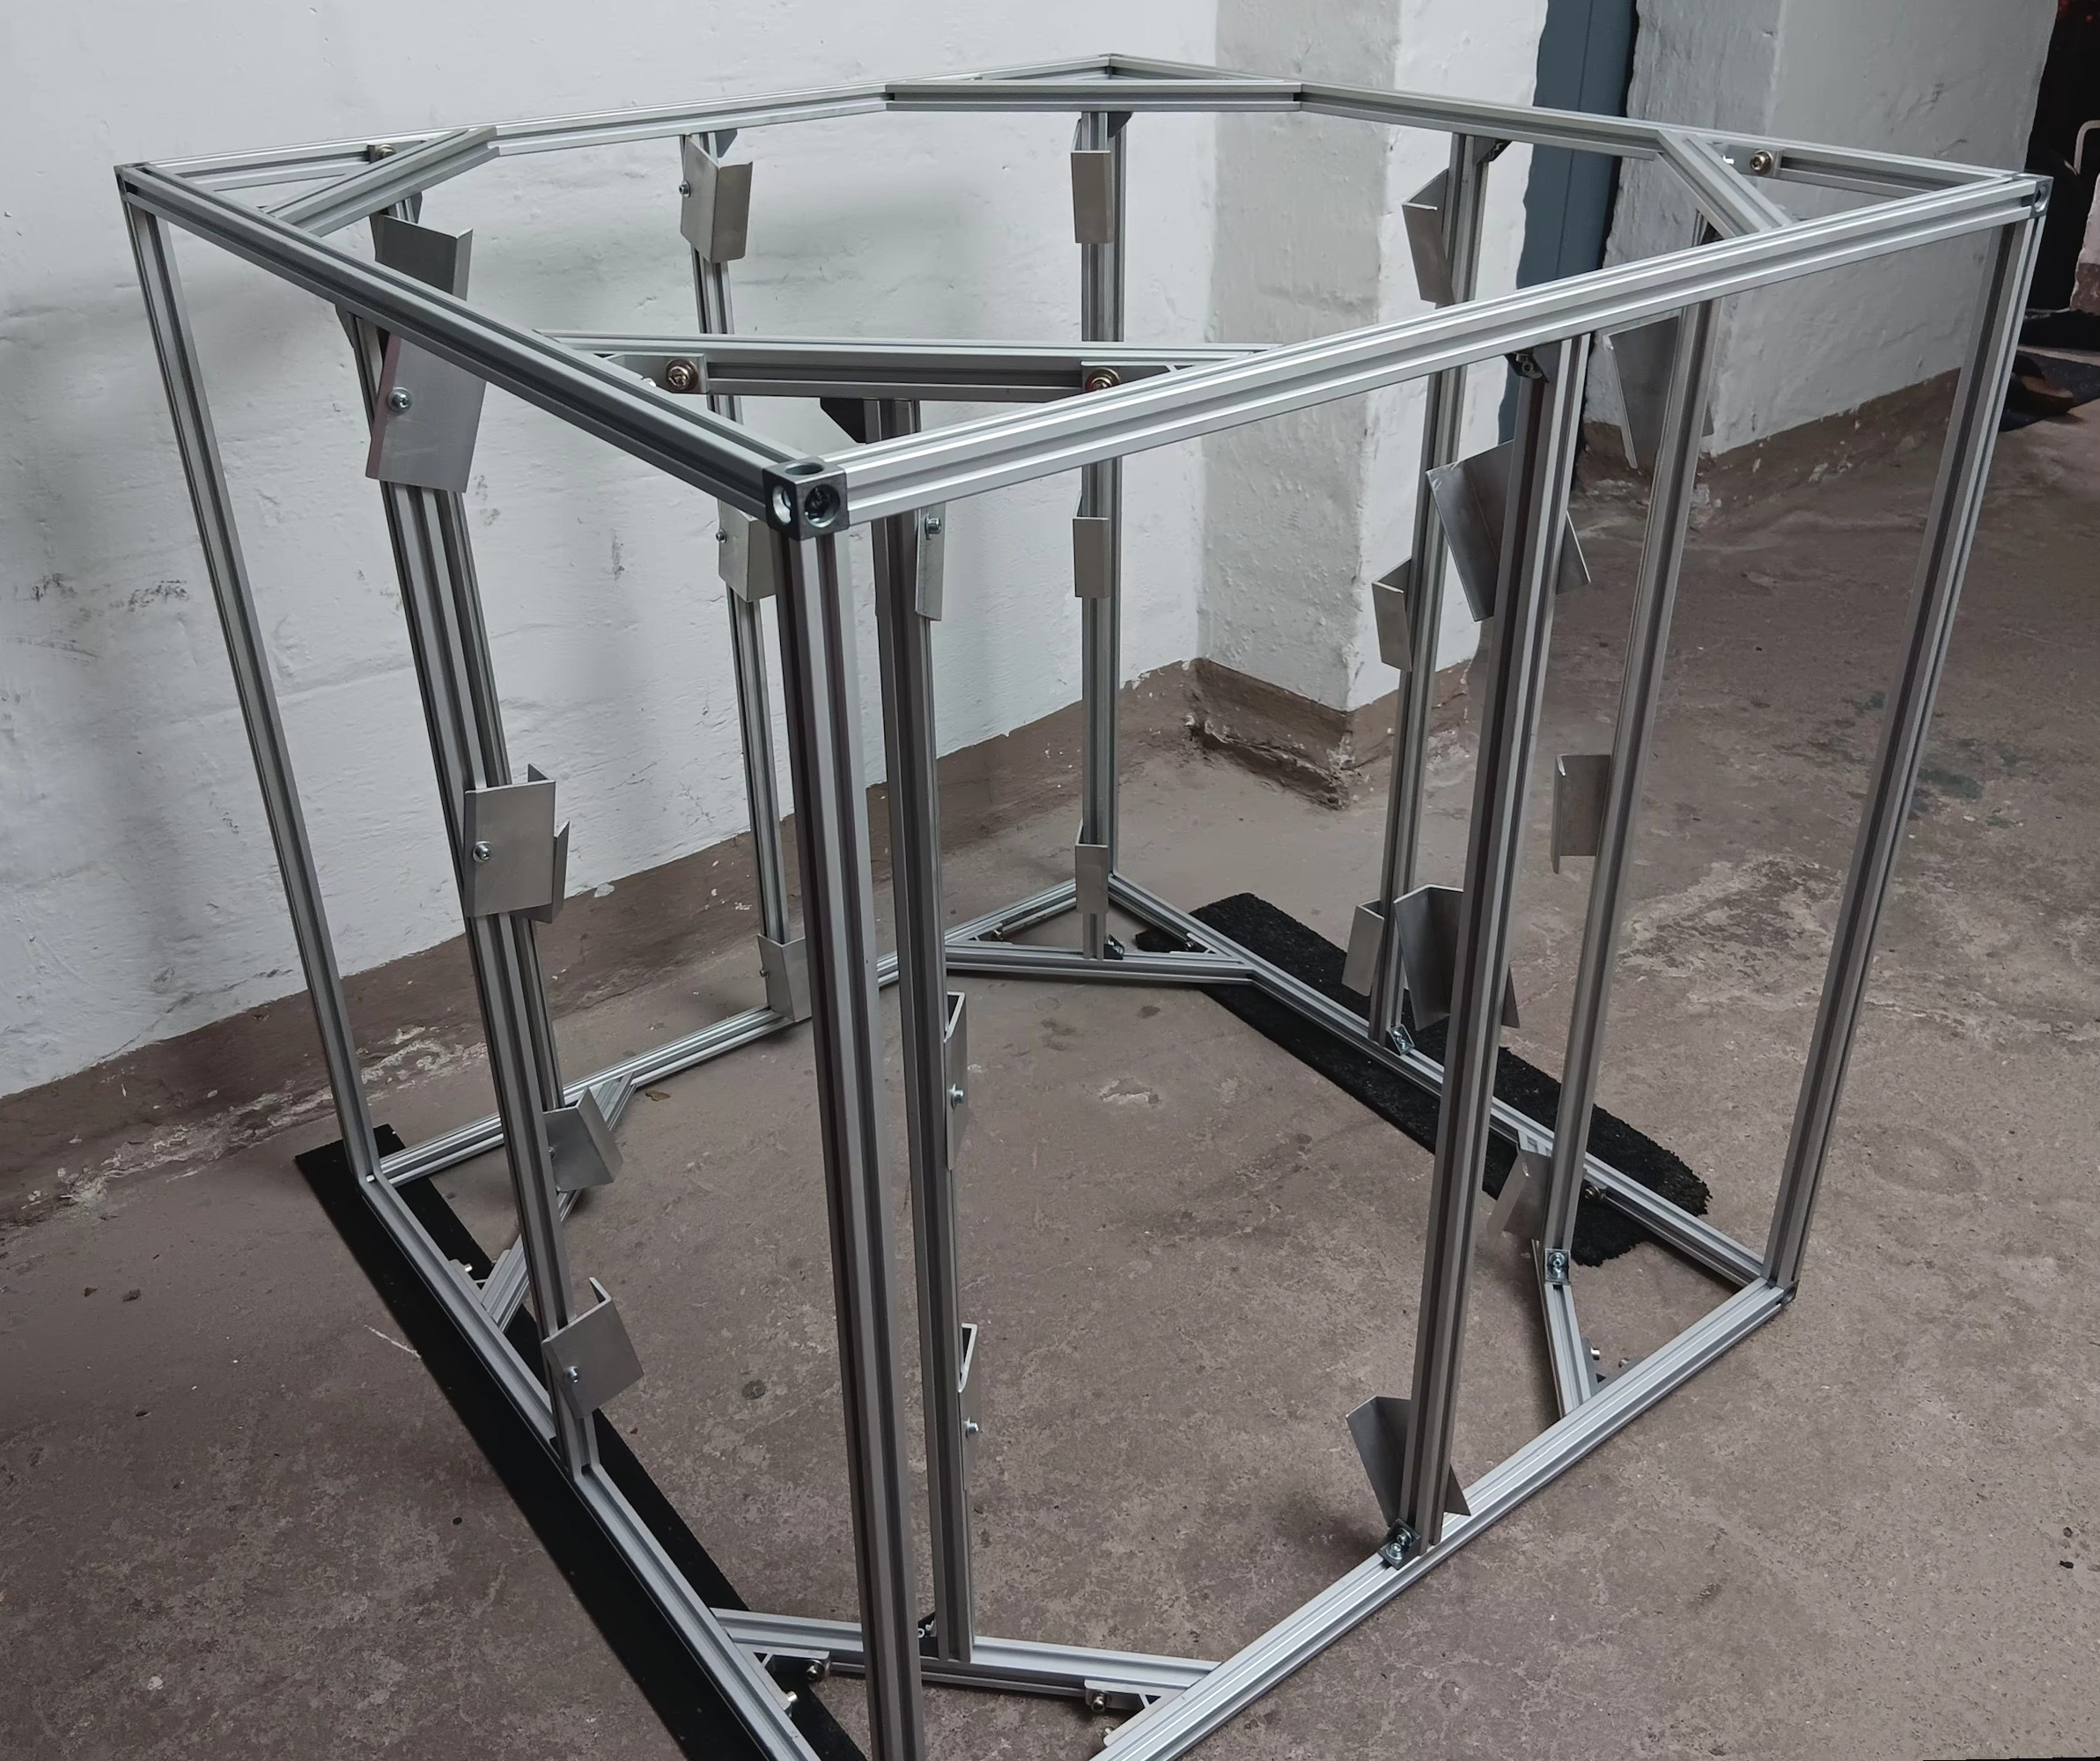
\includegraphics[height=6.5cm]{./img/3_aufbau/alurahmen.jpg}
        \centering
        \caption{Aluminium-Rahmen}
        \label{img:alurahmen} %ID fürs Bder an den Aluprofilen befestigt ist (ild
    \end{subfigure}
    \caption{Alu-Bauteile des Rahmens}
\end{figure}

Die Kameras wurden mit einem $90^\circ$-Winkel am Rahmen montiert, um diese weiterhin noch vertikal schwenken zu können. \autoref{img:aluwinkel} zeigt einen der Winkel, der an den Aluprofilen befestigt wird (noch ohne entsprechende Befestigungsbohrungen).


\section{Beleuchtung}

\begin{figure}
    \centering
    \begin{subfigure}{0.45\textwidth}
        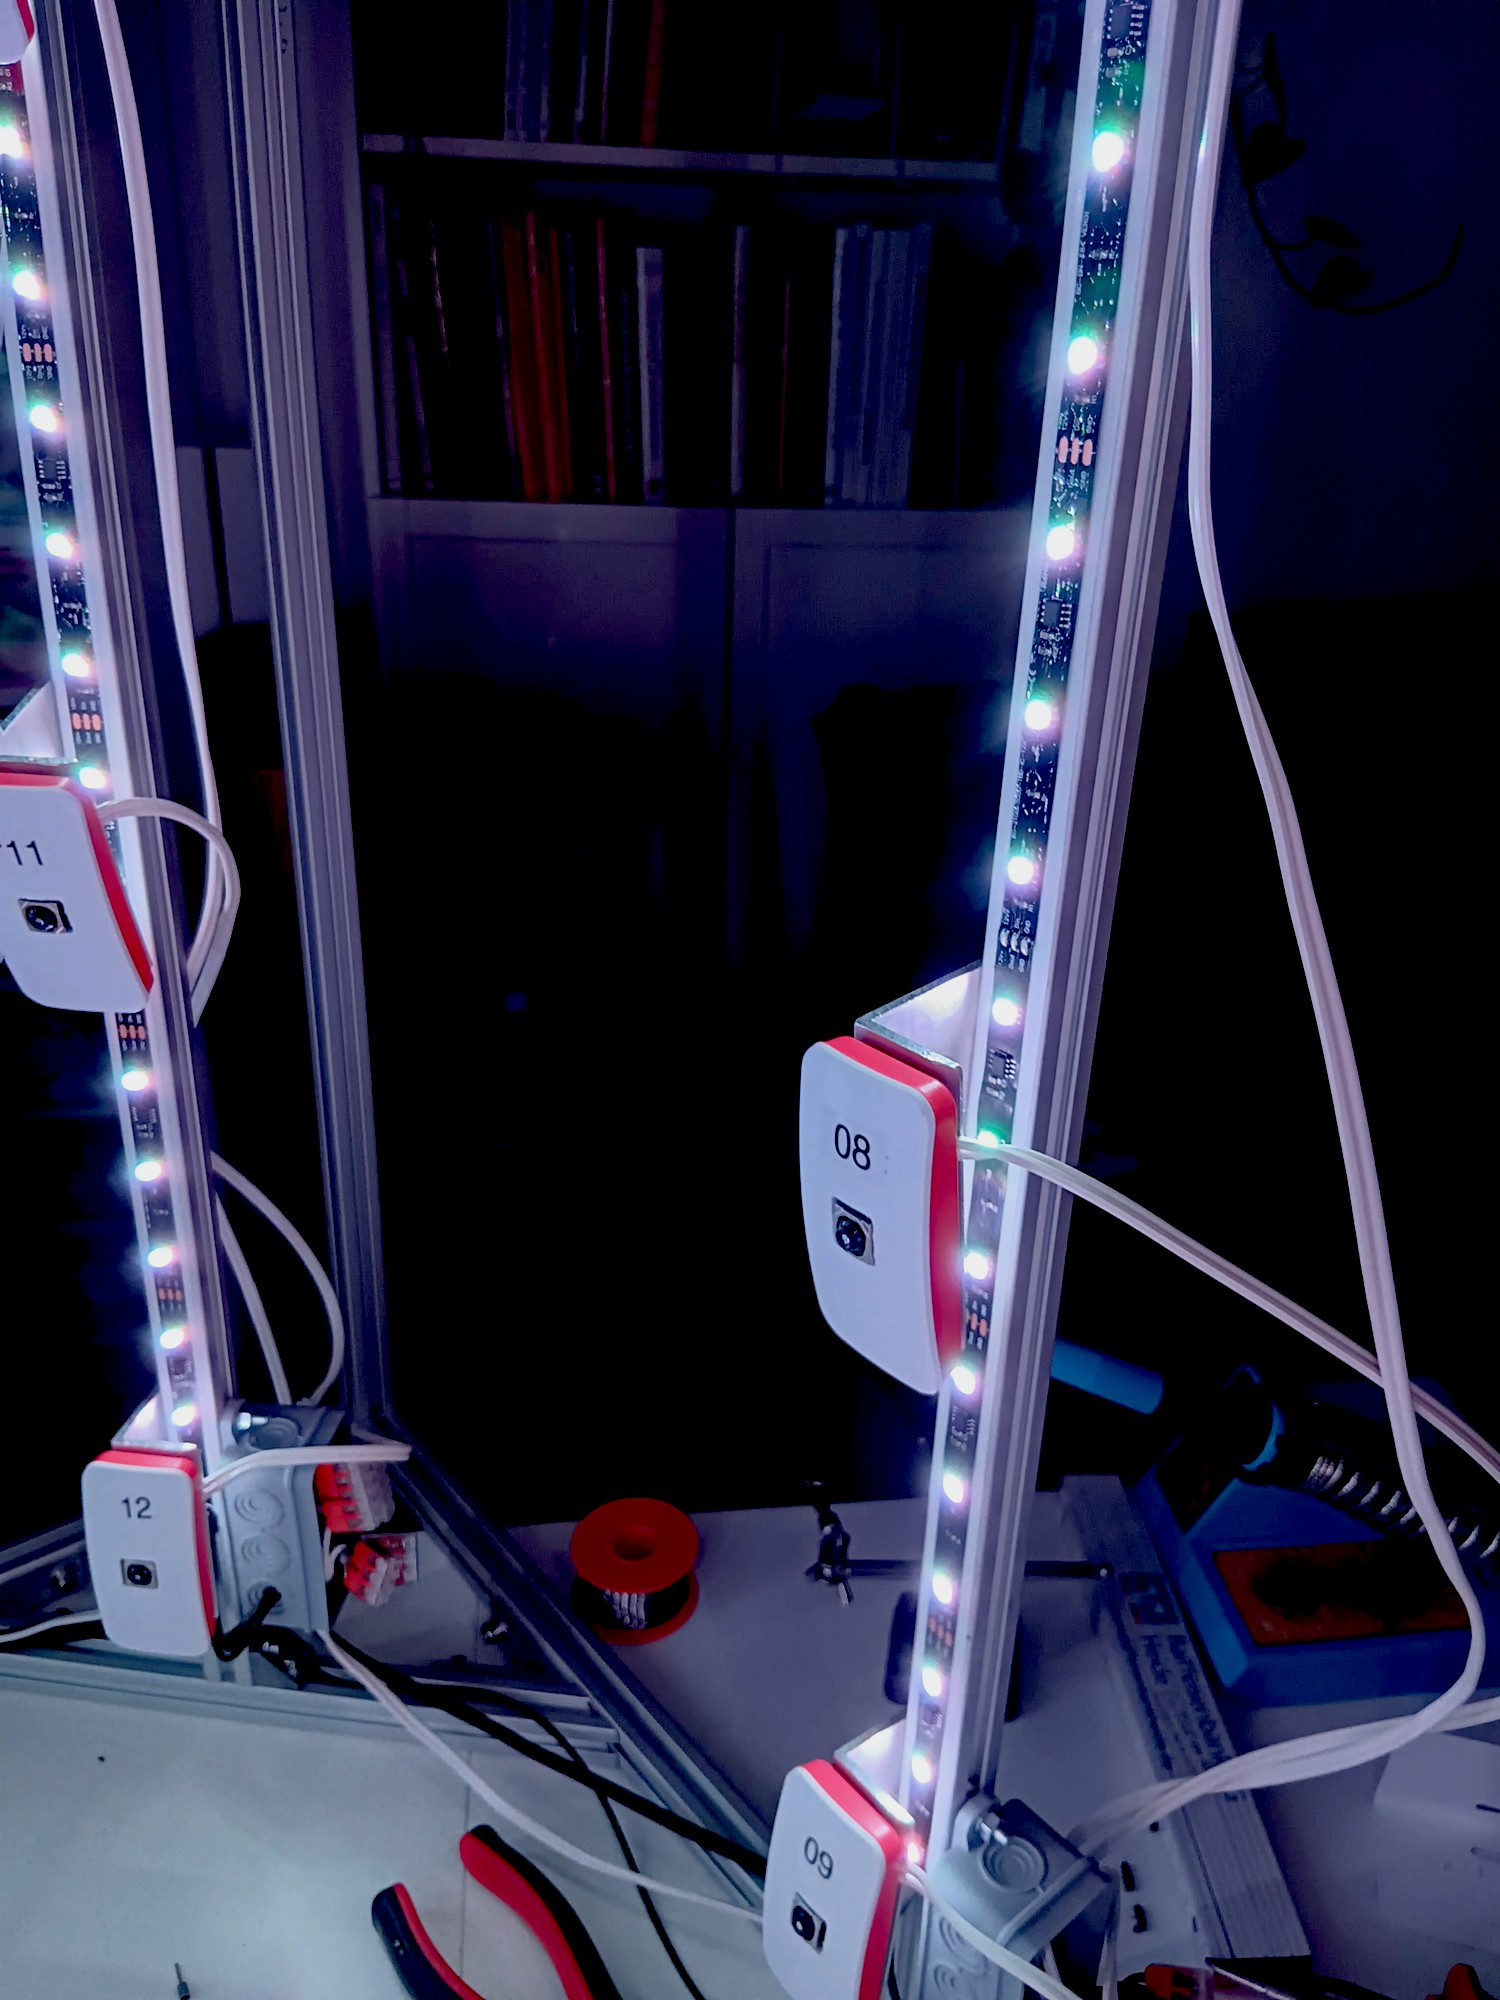
\includegraphics[height=1.2\linewidth]{./img/3_aufbau/beleuchtung.jpg}
        \centering
        \caption{Schattenarme Beleuchtung durch \\LED-Streifen}
        \label{img:led_streifen}
    \end{subfigure}
    \begin{subfigure}{0.45\textwidth}
        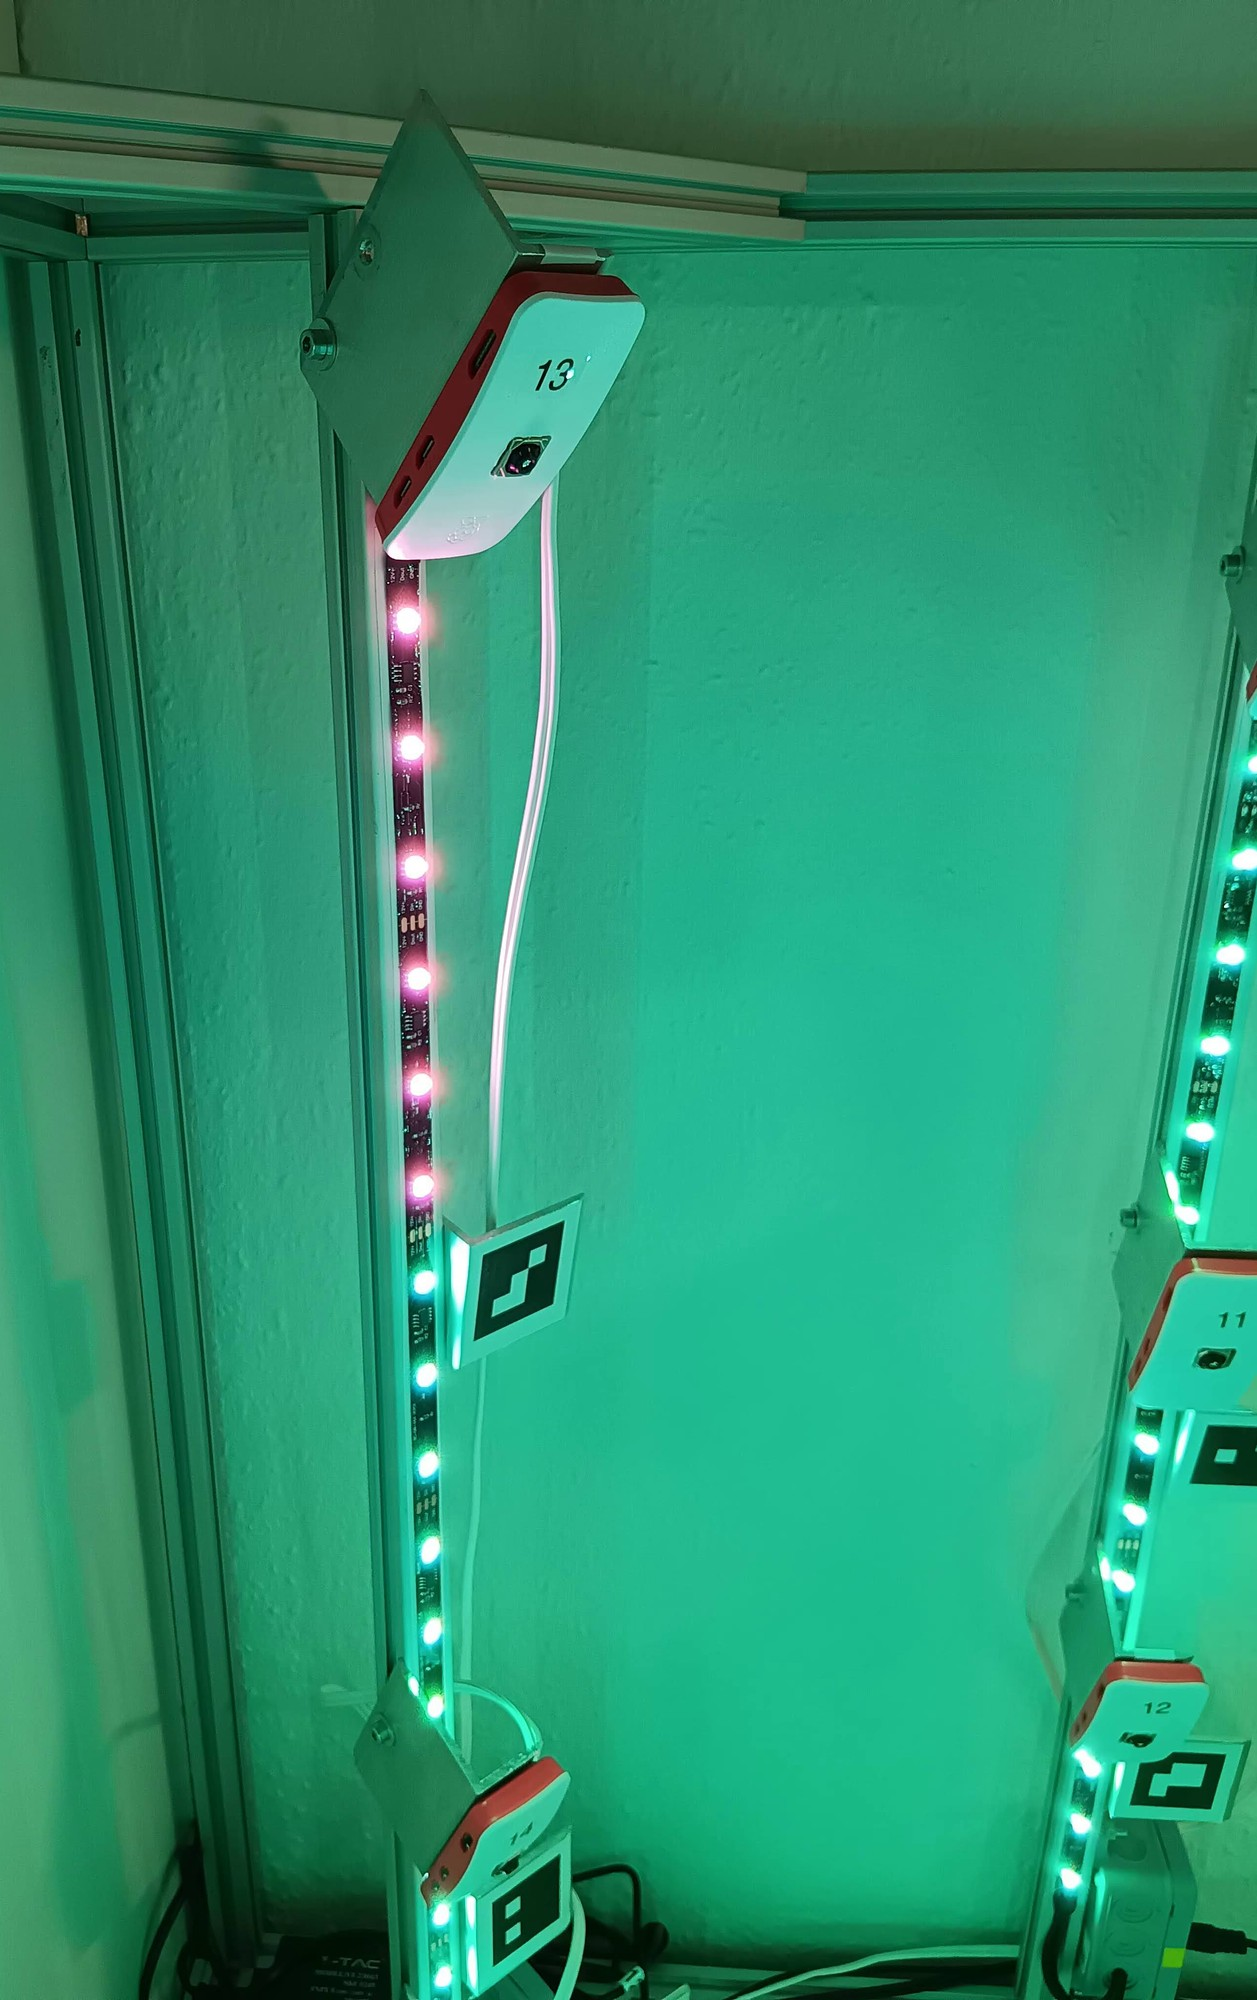
\includegraphics[height=1.2\linewidth]{./img/3_aufbau/beleuchtung_farbig.jpg}
        \centering
        \caption{Farbige Beleuchtung zur\\Statusmeldung}
        \label{img:led_farbig}
    \end{subfigure}
    \caption{Beleuchtung}
\end{figure}

Um möglichst gute Aufnahmen zu erzeugen, sollte das Objekt ausreichend und gleichmäßig ausgeleuchtet sein. Eine dunkle Umgebung verlängert die Belichtungszeit, wodurch die Gefahr von unscharfen Aufnahmen steigt. Schlecht ausgeleuchtete Bereiche (ungleichmäßige Ausleuchtung) verursachen verstärktes Rauschen in diesen Bildbereichen. Problematisch ist bei der Beleuchtung, dass die Kameras ggf. auch die Lichtquellen mit aufnehmen, wodurch Linsenreflexionen oder ein Ausbrennen der Bildbereiche möglich ist. Außerdem störend sind fremde Lichtquellen, die Schatten werfen oder die Belichtung der Kameras beeinflussen können.

Es wurde sich für einzeln steuerbare LED-Lichtstreifen als Lichtquelle entschieden (siehe \autoref{img:led_streifen}). Diese können einfach an den Aluprofilen montiert werden und ermöglichen es, einzelne Bereiche abzuschalten, beispielsweise um Blendwirkungen zu vermindern. Außerdem können hiermit auch verschiedene Lichtfarben eingestellt werden, um Statusmeldungen zu ermöglichen (siehe \autoref{img:led_farbig}) oder ggf. die Farbgebung des Objektes zu beeinflussen. Die Steuerung erfolgt über einen Raspberry Pi 4, der auch die Steuerung der Kameras übernimmt. Die LED-Streifen verfügen hierfür pro drei LEDs über einen integrierten Schaltkreis vom Typ WS2811. Dieser ermöglicht es, jedem Dreier-Verbund über ein proprietäres Steuerprotokoll eine eigene Farbe und Helligkeit zuzuweisen \citep[vgl.][]{ws2811}. Für die Implementierung der Steuerung wurde die Bibliothek \texttt{rpi-ws281x} verwendet, die eine einfache Ansteuerung der LED-Streifen ermöglicht (siehe auch \autoref{p:ws281x}).

Für diffuseres Licht von außen kann ein halbtransparenter, weißer Stoff über den Rahmen gespannt werden. Hierfür wurde aus weißem Baumwollstoff eine entsprechende Haube genäht (siehe \autoref{img:stoffhuelle}), welche durch zwei mittels Reißverschluss verschließbaren Eingriffmöglichkeiten weiterhin das Einlegen von Objekten durch die Seite oder das Verstellen von Kameras ermöglicht (siehe \autoref{img:stoffhuelle_offen}). Diese sorgt für eine gleichmäßigere Ausleuchtung durch Reflexion im Inneren, verhindert Reflexionen an Glasscheiben etc. und vermindert Blendwirkungen durch externe Lichtquellen.


\begin{figure}
    \centering
    \begin{subfigure}{0.45\textwidth}
        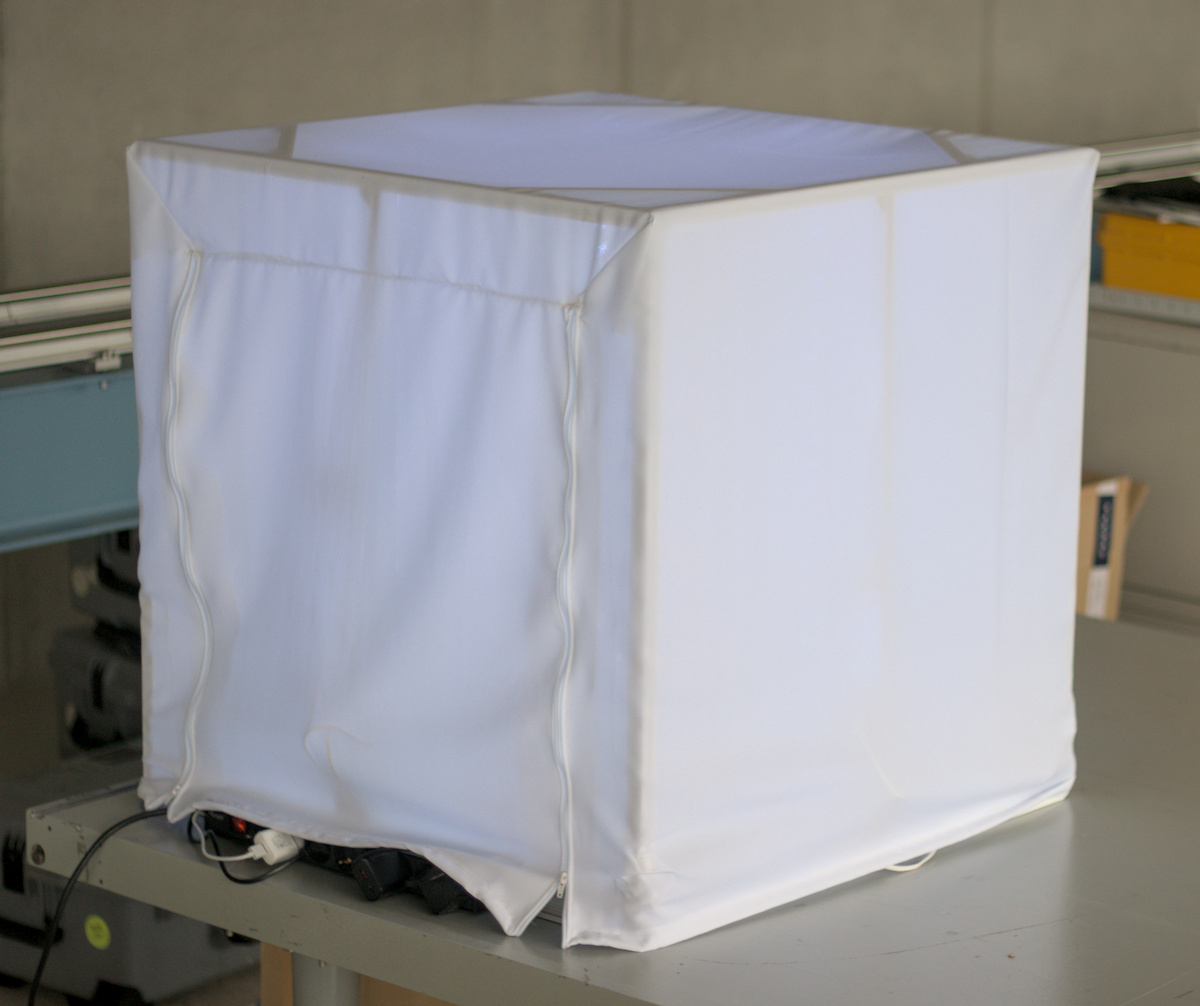
\includegraphics[height=5.2cm]{./img/3_aufbau/stoffhuelle.jpg}
        \centering
        \caption{geschlossene Stoffhülle}
        \label{img:stoffhuelle}
    \end{subfigure}
    \begin{subfigure}{0.45\textwidth}
        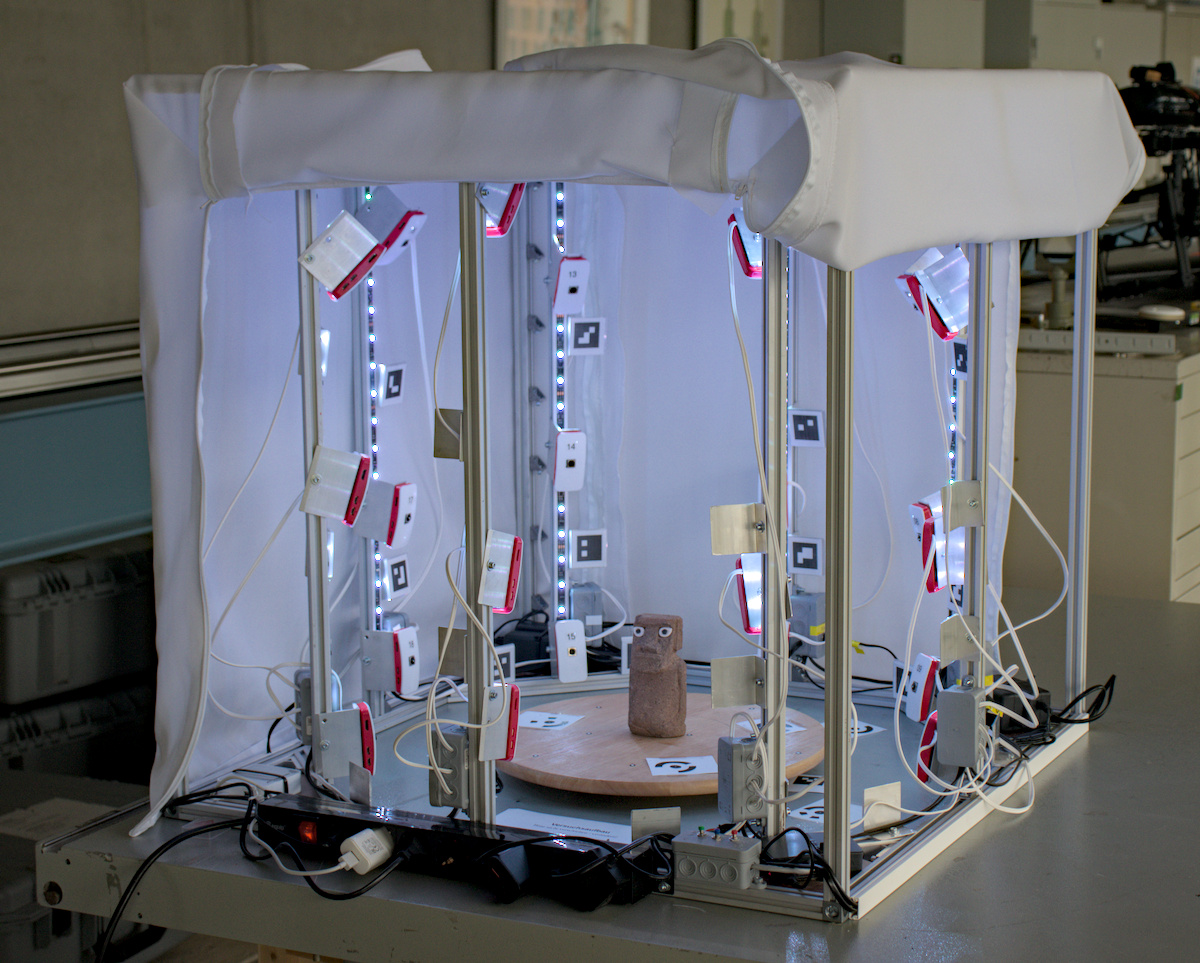
\includegraphics[height=5.2cm]{./img/3_aufbau/stoffhuelle_offen.jpg}
        \centering
        \caption{geöffnete Stoffhülle}
        \label{img:stoffhuelle_offen}
    \end{subfigure}
    \caption{Stoffhülle zur Verminderung von Reflexionen und Blendwirkungen}
\end{figure}

\section{Kommunikation und Datenübertragung}
Die Kommunikation zwischen den Raspberry-Pi-Computern erfolgt über WLAN. Hierfür ist ein Mini-WLAN-Router mit im System verbaut worden. Vorteil dieser Lösung ist, dass hier keine weiteren Leitungen außer der Stromversorgung zu den einzelnen Raspberry Pi Zero W benötigt werden und es auch möglich wäre, die gleiche Hard- und Software für ein größeres System ohne Änderungen zu nutzen. Nachteilig ist die Verbindungsgeschwindigkeit, gerade im Hinblick auf die Synchronisierung der Kameras. Diese Problematik soll aber durch entsprechende Programmierung der Software möglichst klein gehalten werden.

Als weitere Datenleitung wird eine Steuerleitung für die LED-Streifen benötigt. Über diese erfolgt die Steuerung der einzelnen LED-Gruppen. Hier wurde der gleiche Klingeldraht verwendet, der auch für die Stromversorgung (siehe \autoref{sec:strom}) verwendet wird. Sie ist in \autoref{img:schema_energie} in Orange dargestellt.


\section{Stromversorgung}
\label{sec:strom}

\begin{figure}
    \centering
    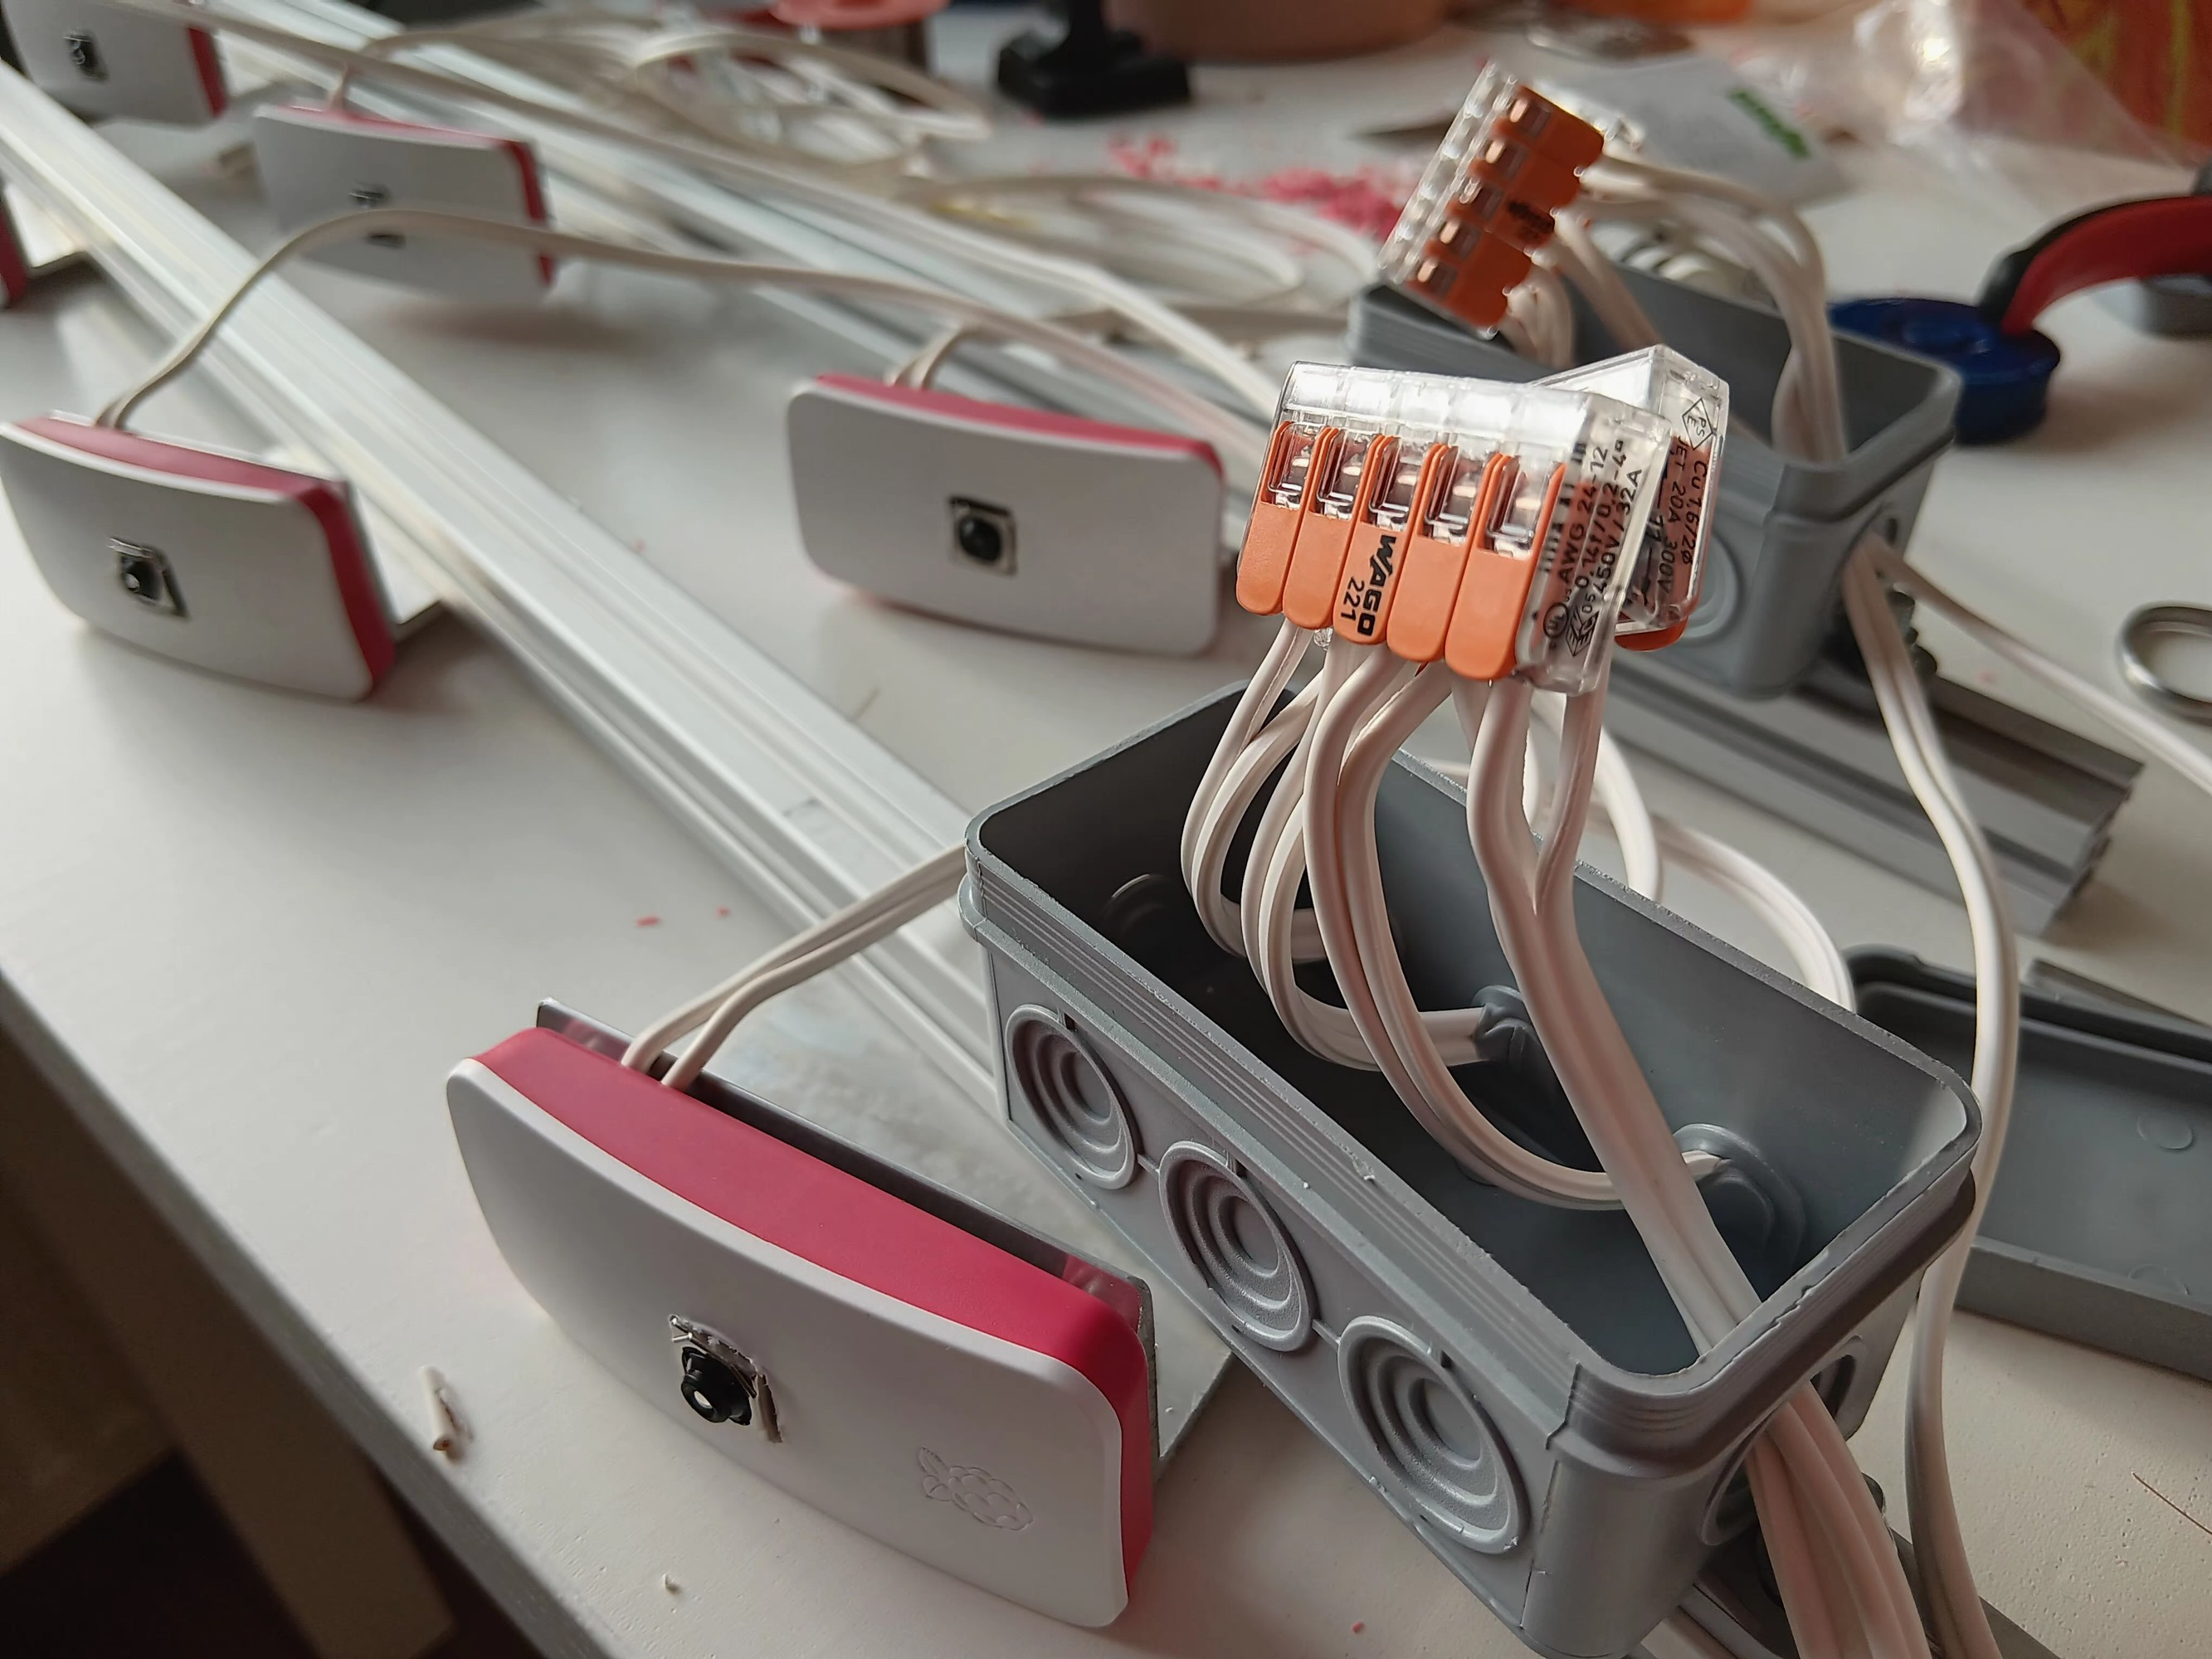
\includegraphics[width=0.7\textwidth]{./img/3_aufbau/stromverteilung.jpg}
    \caption{Elektroverteilung zu den einzelnen Raspberry Pi Zero}
    \label{img:stromverteilung}
\end{figure}

Alle Raspberry-Pi-Computern werden mit \SI{5}{\volt} betrieben. Der Raspberry Pi Zero W mit Kamera hatte dabei in Messungen einen maximalen Stromverbrauch von \SI{270}{\milli\ampere} aufgezeigt, der Raspberry Pi 4 kann bis zu \SI{1,5}{\ampere} unter Last verbrauchen. Hieraus ergibt sich ein Gesamtstromverbrauch von maximal rund \SI{8}{\ampere}. Für den Raspberry Pi 4 wurde ein eigenes 15-Watt-Netzteil eingeplant und für die 24 Raspberry Pi Zero W ein gemeinsames 35-Watt-Netzteil. Versuche zeigten jedoch, dass der Stromverbrauch kurzfristig höher ausfallen kann, sodass die Raspberry Pi Zero W, die am meisten von Spannungsabfällen betroffen sind, zum Absturz gebracht wurden, wenn alle Kameras gleichzeitig auslösten. Nachdem die Last sicherheitshalber auf zwei weitere Netzteile verteilt wurde, lief das System zuverlässig.

Als Kabelmaterial wurde Klingeldraht mit \SI{0,75}{\cubic\milli\metre} verwendet. Der relativ hohe Kabelquerschnitt soll für einen geringen Spannungsabfall sorgen. Durch die Verwendung von mehreren Netzteilen ist dieser jedoch nun nicht mehr notwendig. Hier würde sich nun ein geringerer Querschnitt anbieten, auch um eine einfachere Verbindung zu den Raspberry Pi Zero W zu ermöglichen. Diese wurden aufseiten der Zero W verlötet und in den Verteilerdosen mit Federkraftklemmen verbunden (siehe \autoref{img:stromverteilung}).

Die Stromversorgung der Beleuchtung erfolgt über ein 12-Volt-Netzteil mit \SI{3,5}{\ampere} Ausgangsleistung. Auch hier wurde Klingeldraht zur Verteilung zwischen den einzelnen Holmen genutzt.

Der WLAN-Router wird auch mittels 5-Volt-Gleichspannung betrieben. Hier war ein entsprechendes USB-Netzteil mitgeliefert.

Alle Netzteile werden von einer zentralen Steckdosenleiste mit 230-Volt-Netzspannung versorgt. Sie sind für eine Wechselspannung zwischen $100$ und \SI{230}{\volt} ausgelegt, sodass mit einem entsprechenden Adapter auch eine Nutzung in anderen Ländern möglich wäre. Die gesamte Energieverteilung ist der \autoref{img:schema_energie} zu entnehmen. Rote Verbindungen stellen hierbei 12-Volt-Leitungen dar, blaue 5-Volt-Leitungen und magentafarbene die 230-Volt-Leitungen. Orange Verbindungen sind Datenleitungen (Steuerleitung LED-Streifen).

\begin{figure}
    \centering
    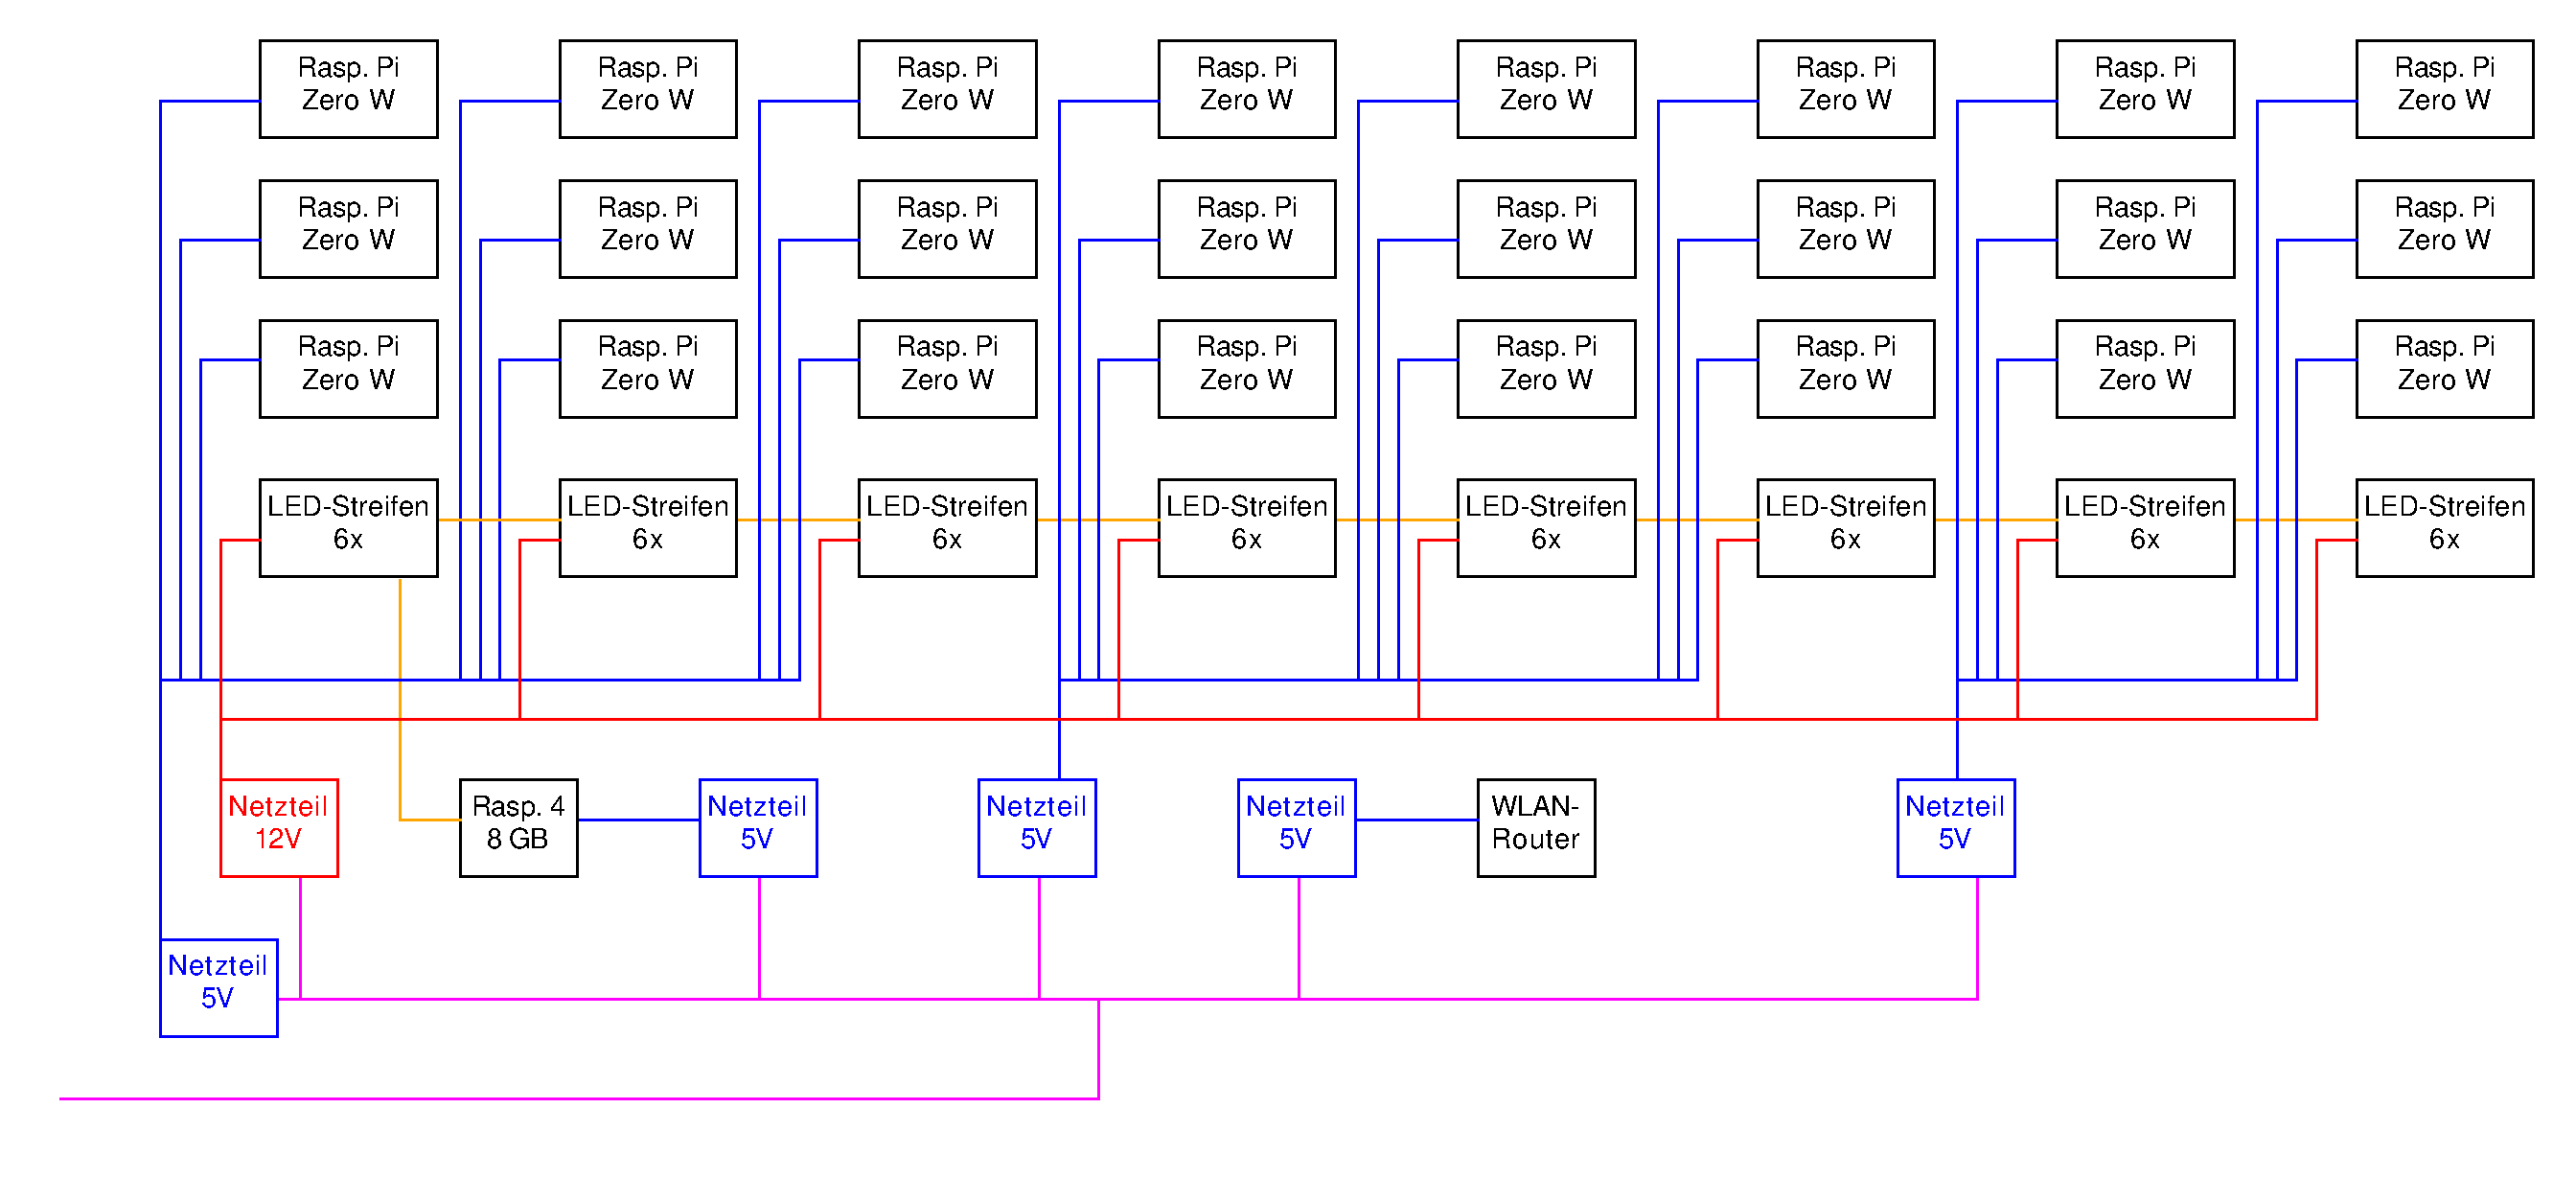
\includegraphics[width=1.\textwidth]{./img/uml/uml_energie.pdf}
    \caption{Schematische Darstellung der Energieversorgung (blau: \SI{5}{\volt}; rot: \SI{12}{\volt}; schwarz: \SI{230}{\volt}; grün: Daten)}
    \label{img:schema_energie}
\end{figure}


\section{Kostenbetrachtung}
Der Titel dieser Arbeit verweist bereits darauf, dass eine kostengünstige Lösung gesucht werden sollte. Während der Konzeption und dem Bau des Systems wurde entsprechend auf einen möglichst gutes Preis-Leistungs-Verhältnis geachtet. Eine Auflistung der Einzelposten ist in \autoref{ch:teileliste} aufgeführt. Die Gesamtkosten betrugen rund 1.800 Euro. Die Kosten für die Softwareentwicklung bzw. der Zeitaufwand dafür sind hier nicht berücksichtigt.

Den größten Teil der Kosten machen die Kameras und die zugehörigen Raspberry-Pi-Computer aus. Wie schon in \autoref{s:kameras} erwähnt, kostet ein Kameramodul etwa 30 Euro. Hierzu kommen noch 18 Euro für den Raspberry Pi Zero W. Mit Gehäuse und Speicherkarte ergeben sich so rund 60 Euro pro Kamera. Für den Prototypen wurden 24 Kameras verwendet, somit entfallen hierauf grob 1.400 Euro und damit über drei Viertel der Gesamtkosten. Die Anzahl der Kameras wird daher auch in \autoref{s:kameraanzahl} auf sein Einsparpotenzial hin untersucht.

Andere elektronische Bauteile verursachten Kosten von rund 200 Euro. Hierzu zählen der Raspberry Pi 4, die Netzteile, der WLAN-Router, die LED-Streifen und die Kabel. Der Rahmen aus Aluminiumprofilen mit Schrauben und Kabelhalterungen kostete rund 150 Euro. Für die Stoffhülle wurden etwa 20 Euro ausgegeben.

Ein nicht zu unterschätzender weiterer Kostenfaktor ist die für den Bau benötigte Zeit. Für den Prototypen wurden, zusammengerechnet rund 2-3 Wochen benötigt. Diese Zeit könnte durch Nutzung von mehr fertigen Bauteilen oder Automatisierung verkürzt werden, dieses würde jedoch wieder höhere Materialkosten zur Folge haben. Auch die Softwareentwicklung, die hier nicht berücksichtigt wurde, verursacht Kosten, die jedoch nicht direkt in die Hardwarekosten einfließen und eher einmaliger Natur sind (Pflegeaufwand ist jedoch zu berücksichtigen).

\biblio
\end{document}